% Magic comments - Informa ao compilador algumas regras de execução, como tipo de compilação ou codificação do texto
% !TeX root = template-abnt-ufop-escola-de-minas.tex
% !TeX encoding = UTF-8
% !BIB TS-program = XeLaTex
% !backend = biber

%% abtex2-modelo-trabalho-academico.tex, v-1.9.2 laurocesar
%% Copyright 2012-2014 by abnTeX2 group at http://abntex2.googlecode.com/
%%
%% This work may be distributed and/or modified under the
%% conditions of the LaTeX Project Public License, either version 1.3 of this license or (at your option) any later version.
%%
%% This work has the LPPL maintenance status `maintained'.
%%
%% INÍCIO DAS CUSTOMIZAÇÕES PARA A UNIVERSIDADE FEDERAL DE OURO PRETO%%

%% 2022.3.30 13h15 Danny Tonidandel
%% Altera as definições de capa, alterando  o comando, inserindo figuras próprias da Universidade e alterando a disposição dos elementos na contra-capa
%% Remove itens de abstract em francês
%% Altera disposição dos elementos na folha de aprovação
%% Altera o conteudo dos capítulos para um arquivo único.
%% Personalização do estilo biblatex-abnt para adequação à normaABNT 6023:2018
% Reseta contadores das notas de rodapé em cada capítulo
% Insere comandos para exibir uma caixa colorida de fundo cinza para notas explicativas, à escolha do autor

%% 2017.5.31 21h13 Danny Tonidandel
%% Altera nome de arquivo de logomarca
%% remove resumos em espanhol e italiano
%% Insere exemplos para elaboração de tabelas
%% Insere tabela de cronograma de atividades (para projeto de pesquisa)

%% FIM DAS CUSTOMIZAÇÕES PARA A UNIVERSIDADE FEDERAL DE OURO PRETO

%% This work consists of the files
% template-abnt-ufop-escola-de-minas.tex
% referencias.bib
%%
% --------------------------------------------
% ----------------------------------------------
% abnTeX2: Modelo de trabalho Academico (tese de doutorado, dissertacao de

% mestrado e trabalhos monograficos em geral) em conformidade com
% ABNT NBR 14724:2011: Informacao e documentacao - Trabalhos academicos -
% Apresentacao
% ------------------------------------------------------------------------
% ------------------------------------------------------------------------

\documentclass[
	% -- opções da classe memoir --
	12pt,				% tamanho da fonte
	openright,			% capítulos começam em pág ímpar (insere página vazia caso preciso)
	oneside,			% p/ impressão verso e anverso: twoside
	a4paper,			% tamanho do papel.
	% -- opções da classe abntex2 --
	%chapter=TITLE,		% títulos de capítulos convertidos em letras maiúsculas
	%section=TITLE,		% títulos de seções convertidos em letras maiúsculas
	%subsection=TITLE,	% títulos de subseções convertidos em letras maiúsculas
	%subsubsection=TITLE,% títulos de subsubseções convertidos em letras maiúsculas
	% -- opções do pacote babel --
	english,			% idioma adicional para hifenização
	brazil				% o último idioma é o principal do documento
	]{abntex2}

% ---
% Pacotes básicos
% ---

\usepackage{graphicx} 	% gráficos
\usepackage[table,xcdraw]{xcolor}	% tabelas
\graphicspath{{figuras/}} % pasta para figuras
\DeclareGraphicsExtensions{.pdf,.eps,.svg,.png,.jpg,.bmp}

\usepackage{indentfirst} % para identação no primeiro parágrafo
\usepackage{booktabs}
\usepackage{microtype} 	% justificação
\usepackage{verbatim}

% Pacotes de escrita matemática
\usepackage{amsmath,amssymb,unicode-math}


\usepackage{pdfpages} %  anexar pdf diretamente no documento
\usepackage{csquotes}

% Citações


% Opção 2: notas explicativas no sistema autor-data
\usepackage[backend=biber,
% % configuracoes do estilo abnt
 style=abnt,
 sccite, % sobrenomes em caixa alta
 ittitles, % Titulos em italico
 citecount, % contar o número de citações
 scbib, % biliografia em caixa alta
 justify, % alinhamento justificado
 noslsn,
 repeatfields,
 sorting=nty, % ordem alfabetica
 ]{biblatex}

% ARQUIVO COM AS REFERÊNCIAS BIBLIOGRAFICAS
\addbibresource{referencias.bib}

% ---
% Personalização do estilo biblatex-abnt
%Danny A. V. Tonidandel

% Adequa as urls de acordo com normas 6023:2018
\DeclareFieldFormat{url}{\bibstring{urlfrom}\addcolon\addspace \url{#1}}%
\DeclareFieldFormat{urldate}{\bibstring{urlseen}\addcolon\addspace #1}%

% Reseta contadores das notas de rodapé em cada capítulo
\makeatletter
\@addtoreset{footnote}{chapter}
\makeatother

% Pacotes adicionais - podem ser comentados
\usepackage{lipsum}	% para geração de texto aleatório
% ---


% ---
% Informações de dados para CAPA e FOLHA DE ROSTO
% ---
\titulo{Atitude e Controle de Satélites Artificias}
\autor{Vitor Augusto Otoni Figueiró}
\local{Ouro Preto}
\data{\the\year} % imprime o ano corrente no campo data
\orientador{Prof. João Carlos Vilela Castro.}
\coorientador{-}
\instituicao{Universidade Federal de Ouro Preto}
\tipotrabalho{Monografia de Graduação}
\preambulo{Trabalho apresentado ao Colegiado do Curso de Engenharia de Controle e Automação da Universidade Federal de Ouro Preto como parte dos requisitos para a obtenção do Grau de Engenheiro(a) de Controle e Automação.}
% ---


% ---
% Aparência do PDF final

% alterando o aspecto da cor azul
\definecolor{blue}{RGB}{41,5,195}

% informações do PDF
\makeatletter
\hypersetup{
     	%pagebackref=true,
		pdftitle={\@title},
		pdfauthor={\@author},
    	pdfsubject={\imprimirpreambulo},
	    pdfcreator={LaTeX with abnTeX2},
		pdfkeywords={ufop}{latex}{decat}{monografia},
		colorlinks=true,   % opções: false, true
    	linkcolor=blue,    % cor de links internos
    	citecolor=blue,    % cor de links na bibliografia
    	filecolor=magenta, % color de links para arquivos
		urlcolor=blue,     % cor de hiperlinks (urls)
}
\makeatother
% ---

% ---
% Espaçamentos entre linhas e parágrafos
% ---

\setlength{\parindent}{1.3cm} % Tamanho do parágrafo


\setlength{\parskip}{0.2cm} % Espaçamento entre parágrafos
% tente também \onelineskip


\makeindex % compila o indice


\begin{document} % Início do documento

\frenchspacing % Retira espaço obsoleto

% Pré-TextualEXTUAIS
% \pretextual

% Capa - obrigatório

\begin{capa}
	\thispagestyle{empty}
		\centering
	\begin{center}
		\begin{minipage}{1\linewidth}
			\centering
			\begin{tabular}{ccc}
				\begin{tabular}{c}
					\\
					
\includegraphics[width=0.9cm]{logo-universidade.jpg}
				\end{tabular}
				&
				\begin{tabular}{c}
					\\
					{\large \imprimirinstituicao} \\
					{\large Escola de Minas} \\
					{\large CECAU - Colegiado do Curso de } \\
					{\large Engenharia de Controle e Automação}
				\end{tabular}
				&
				\begin{tabular}{c}
					\\
					
\includegraphics[width=2.1cm]{logo-unidade-2.jpg}
				\end{tabular}
			\end{tabular}
		\end{minipage}

\centering
\vspace*{1cm}
{\ABNTEXchapterfont\large\imprimirautor}
\vspace*{\fill}

{\ABNTEXchapterfont\bfseries \large \imprimirtitulo}
\vspace*{\fill}

{\large\imprimirtipotrabalho}
\vspace*{\fill}

{\large\imprimirlocal}, {\large \the\year}
%\par
\vspace*{1cm}
	\end{center}
\end{capa}



% Folha de rosto [OBRIGATÓRIO]
\imprimirfolhaderosto
 %\imprimirfolhaderosto* se quiser ficha catalográfica

% Ficha bibliográfica [OPCIONAL,segundo determinação CECAU  e DECAT, 29/03/2023]
% \begin{fichacatalografica}
  %   \includepdf{fig_ficha_catalografica.pdf}
% \end{fichacatalografica}


% Folha de aprovação - Obrigatório NBR 14724/2011
%\begin{folhadeaprovacao}
%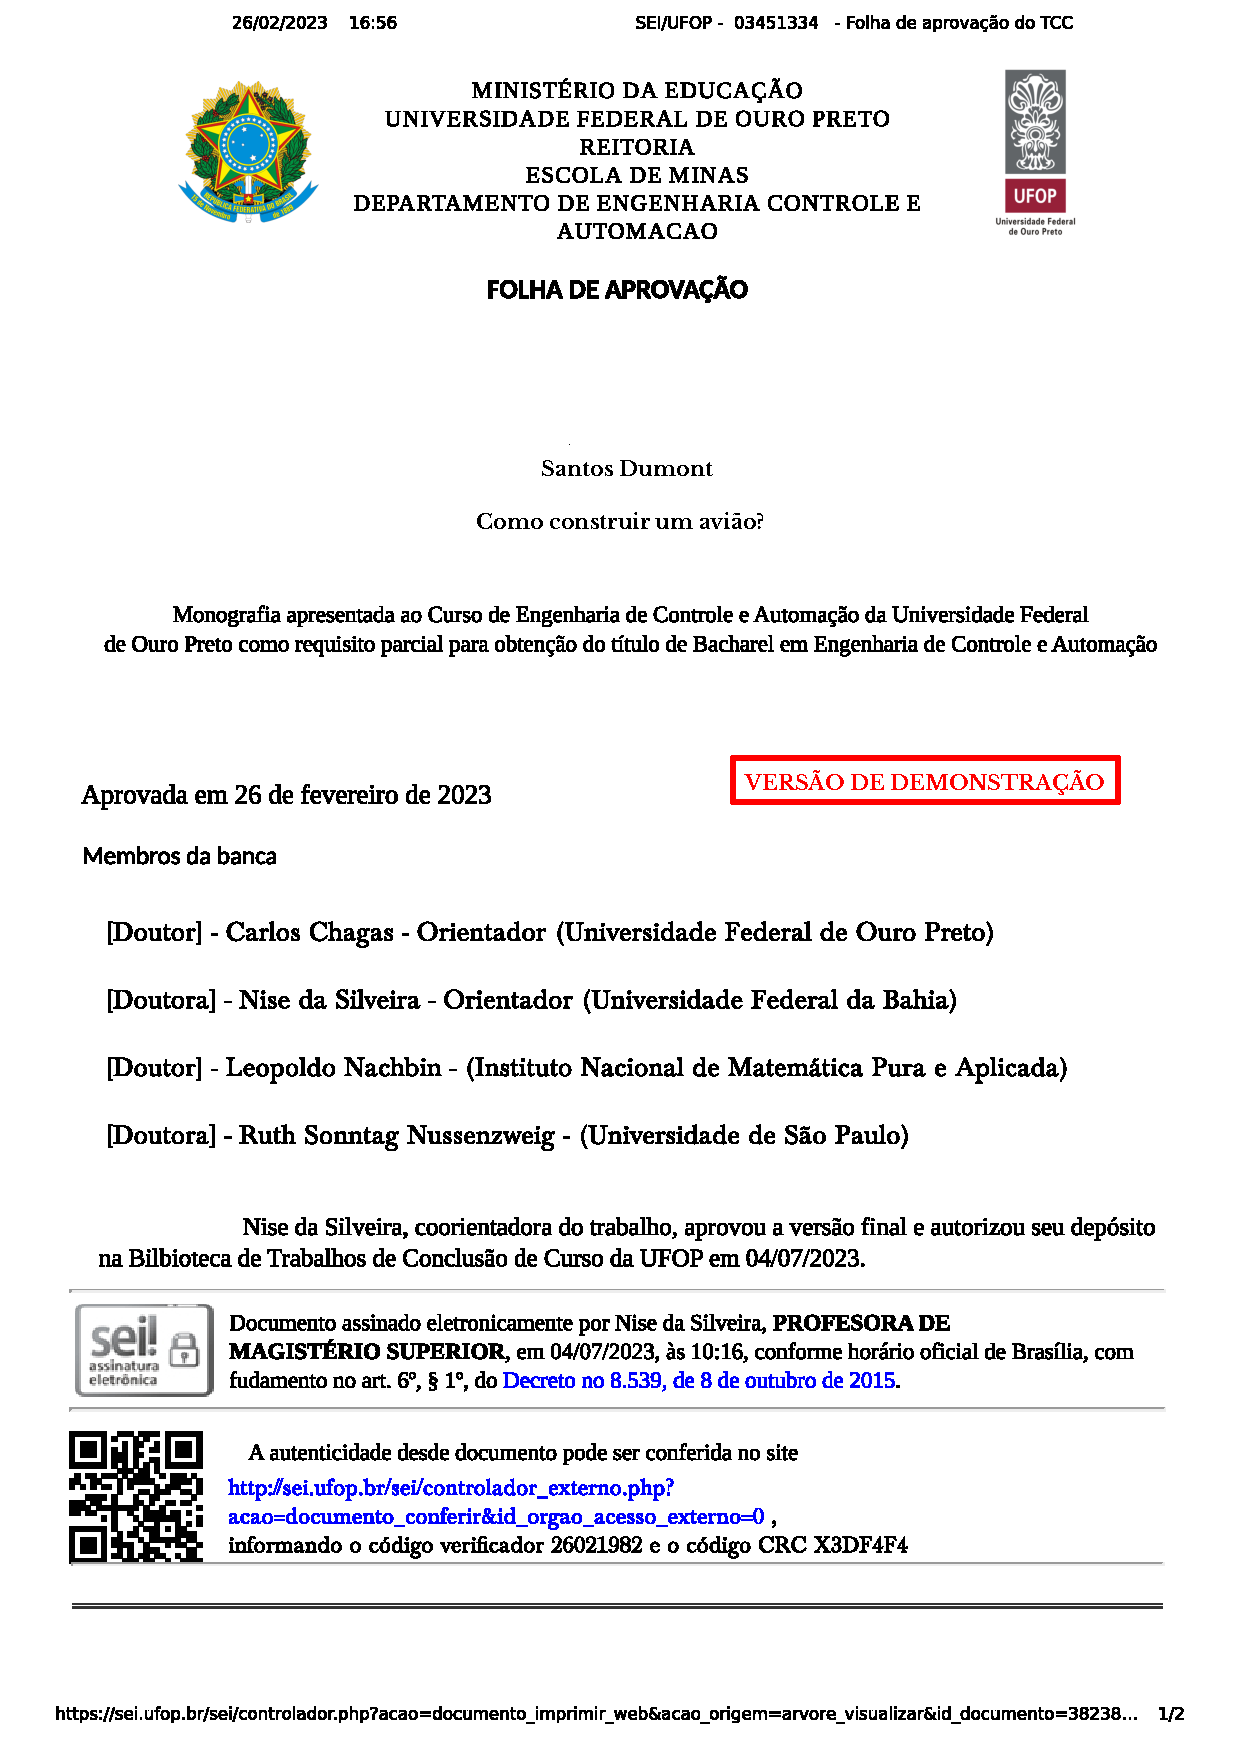
\includepdf{folha-de-aprovacao.pdf}
%\end{folhadeaprovacao}


% Agradecimentos - opcional
\begin{agradecimentos}
\noindent Os agradecimentos [são opcionais, e] vem aqui...
\end{agradecimentos}

% Epígrafe - Opcional
\begin{epigrafe}
    \vspace*{\fill}
\epigraph{\textsl{Júpiter leva 4332 dias para fazer uma revolução.}}{---~Oliver Lodge.}
\end{epigrafe}
% ---

% ---
% RESUMOS
% ---

% resumo em português
\setlength{\absparsep}{18pt} % ajusta o espaçamento dos parágrafos do resumo
\begin{resumo}
 %\noindent O resumo deve ressaltar o objetivo, o método, os resultados e as conclusões do documento. A ordem e a extensão destes itens dependem do tipo de resumo (informativo ou indicativo) e do tratamento que cada item recebe no documento original. O resumo deve ser precedido da referência do documento, com exceção do resumo inserido no próprio documento. (\ldots) As palavras-chave devem figurar logo abaixo do resumo, antecedidas da expressão Palavras-chave:, separadas entre si por ponto e finalizadas também por ponto.
Os satélites artificiais desempenham um papel essencial em diversos setores, como comunicação, monitoramento ambiental, sensoriamento remoto e pesquisa científica. Para que esses satélites cumpram suas funções corretamente, é necessário que mantenham uma orientação adequada em relação à Terra ou a outros objetos de interesse. Isso é feito por meio de sistemas de controle de atitude. Este trabalho tem como objetivo o desenvolvimento de um sistema de estimação e controle de atitude de satélites artificiais, especificamente para CubeSats, utilizando sensores inerciais e um microcontrolador ESP32. A metodologia adotada incluiu a revisão bibliográfica sobre conceitos fundamentais como ângulos de Euler, quatérnions e matrizes de rotação, além da implementação de algoritmos de determinação de atitude.


 \textbf{Palavras-chaves}: controle de atitude. CubeSat. ESP32. sensores inerciais.
\end{resumo}

% resumo em inglês
\begin{resumo}[Abstract]
 \begin{otherlanguage*}{english}

\noindent Artificial satellites play a crucial role in various sectors such as communication, environmental monitoring, remote sensing, and scientific research. For these satellites to perform their functions correctly, they must maintain an appropriate orientation relative to Earth or other objects of interest. This is achieved through attitude control systems. This work aims to develop an attitude estimation and control system for artificial satellites, specifically CubeSats, using inertial sensors and an ESP32 microcontroller. The adopted methodology included a bibliographic review of fundamental concepts such as Euler angles, quaternions, and rotation matrices, in addition to the implementation of attitude determination algorithms.

   \vspace{\onelineskip}

   \noindent
   \textbf{Key-words}: attitude control. CubeSat. ESP32. inertial sensors
 \end{otherlanguage*}
\end{resumo}


% Lista de ilustrações
\pdfbookmark[0]{\listfigurename}{lof}
\listoffigures*
\cleardoublepage
% ---

% inserir lista de tabelas
\pdfbookmark[0]{\listtablename}{lot}
\listoftables*
\cleardoublepage
% ---

% ---
% Lista de abreviaturas e siglas [OPCIONAL]
% ---

\begin{siglas}
  \item[CI] Circuito Integrado 
  \item[IMU] Unidade de Medição Inercial
\end{siglas}
% ---

%---
% Lista de símbolos [OPCIONAL]
%---
%\begin{simbolos}
  
%\end{simbolos}
% ---

% ---
% Sumário
% ---
\pdfbookmark[0]{\contentsname}{toc}
\tableofcontents*
\cleardoublepage


% Reinicia contadores das notas de rodapé
\makeatletter
\@addtoreset{footnote}{chapter}
\makeatother



% ELEMENTOS TEXTUAIS

\textual

% Modelo de capitulo com a introducao, objetivos e estrutura do texto

% --
\chapter[Introdução]{Introdução}



Os satélites artificiais desempenham um papel fundamental em interações com a Terra, corpos celestes ou outros artefatos espaciais, realizando tarefas essenciais por meio de instrumentos e dispositivos que precisam ser posicionados e orientados corretamente para garantir o desempenho ideal \cite{shuster1993} \textit{apud} \cite{ferreira2008}. Um exemplo notável desse tipo de tecnologia é o Sputnik 1. No dia 4 de outubro de 1957, o a aeronave foi lançada com sucesso, tornando-se o primeiro objeto feito pelo homem a entrar na órbita da Terra e marcando o início da 'Era Espacial' (ver Figura \ref{fig:sputnik}). 

\begin{figure}[h]
	\centering
	\includegraphics[scale=0.6]{Sputnik.jpg} % ajuste o valor do scale conforme necessário
	\caption[Sputnik 1 antes do lançamento em outubro de 1957]{Sputnik 1 antes do lançamento em outubro de 1957}
	\fonte[Fonte: European Space Agency (ESA). Disponível em:]{\url{https://www.esa.int/ESA_Multimedia/Images/2007/10/Sputnik_1_before_launch_in_October_1957}}
	\label{fig:sputnik}
\end{figure}

A determinação de atitude, que corresponde à orientação de um veículo espacial em relação a um referencial inercial ou a um objeto de interesse, como a Terra, é um processo essencial para o controle dessas missões. Este processo, normalmente realizado por sensores de alta precisão e algoritmos sofisticados de processamento de dados, garante que o satélite se mantenha na posição correta. A precisão da determinação de atitude depende da combinação dos métodos de processamento aplicados e do hardware utilizado. Em resumo, determinar a atitude de um satélite significa calcular sua matriz de atitude em relação a um referencial previamente estabelecido \cite{Wertz2012}.

A atitude de um satélite, ou seja, sua orientação no espaço, é crucial para o sucesso de missões espaciais. Como destacado por \cite{YANG2012198}, "A determinação e controle da atitude de um satélite é uma parte importante para que o satélite alcance sua missão projetada", sendo este controle um fator determinante no desempenho de satélites já lançados. Yang também ressalta que "A determinação da atitude é muito importante por duas razões: primeiro, os engenheiros de controle precisam verificar se a orientação está correta; segundo, se não estiver, o erro é comparado com a atitude desejada e utilizado para ajustar os atuadores, corrigindo a orientação do satélite".

Com a crescente demanda por satélites dedicados a comunicação, monitoramento ambiental, sensoriamento remoto e pesquisa científica, o controle preciso da atitude tornou-se indispensável. O sucesso dessas missões depende da capacidade de manter a eficiência e a precisão operacionais, especialmente em um cenário de crescente complexidade tecnológica e competitividade no setor aeroespacial.

Os dados coletados pelos sensores de atitude, normalmente representados como componentes vetoriais, podem ser apresentados em diversas formas, como quatérnions, ângulos de Euler ou matrizes de rotação. Os quatérnions, por exemplo, oferecem uma forma concisa e eficiente de descrever a rotação, permitindo uma interpretação geométrica clara do eixo e do ângulo de rotação \cite{jia2013quaternions}, enquanto os modelos de ângulos de Euler têm se mostrado muito eficientes porque os modelos linearizados baseados nesses ângulos são controláveis, e todos os métodos padrão de projeto de sistemas de controle lineares são diretamente aplicáveis\cite{YANG2012198}. As matrizes de rotação, por sua vez, é explicada como uma ferramenta usada para descrever a rotação de um objeto no espaço tridimensional em relação a um sistema de coordenadas inercial. Essa matriz é derivada a partir de ângulos de Euler e é usada para transformar coordenadas de um sistema de referência para outro. A matriz resultante é aplicada em diversas operações que envolvem a orientação espacial de satélites, como a determinação da atitude \cite{silva2016}


%A determinação da atitude de um satélite é essencial não só para garantir o bom funcionamento do controle de atitude, mas também para assegurar a precisão e confiabilidade dos dados coletados pelo satélite
  

\section{Justificativas e Relevância}

a escrever

\section{Metodologia}
Foi realizada no período de 4 meses, uma revisão bibliográfica, que teve como objetivo, estudar sistemas fotovoltaicos para aplicações aeroespaciais, topologias de conversores eletrônicos de potência, estratégias de controle e gerenciamento de energia, baterias e sistemas de acumulação de energia, medições em sistemas aeroespaciais e algoritmos para estimação de atitude, afim de definir um projeto preliminar para a unidade de processamento, condicionamento e regulação de energia fotovoltaica com sistema de estimação de atitude integrado e desenvolver modelos matemáticos. 

No início do projeto, projetamos o desenvolvimento de uma plataforma para determinar a atitude do satélite, mas antes disso, se fez necessário definirmos quais seriam os objetivos a serem alcançados com a utilização de tal plataforma. Alguns desses objetivos seguem a ideia trabalhada em \cite{tavares2017}"Fazer a leitura da orientação atual apresentada pelo satélite, processar os algoritmos necessários, gerar a matriz de atitude do objeto que o relaciona com uma referência conhecida".

Antes de criarmos uma estrutura física, para o teste dos sensores e do funcionamento dos algoritmos implementados, criou-se um código em Python que através da leitura dos sensores e do processamento do algoritmo de determinação da atitude, gera como resposta um objeto 3D, que se orienta no espaço através dos valores lidos pelo sensores, conforme visto nas figuras \ref{fig:Imagemcubo1} e \ref{fig:Imagemcubo2}.

Os algoritmos de medição, estimação e controle foram implementados em uma plataforma programável baseada em um microcontrolador, capaz de realizar a aquisição e o processamento de sinais analógicos e digitais. Essa solução oferece um desempenho satisfatório em tempo real, garantindo a resposta rápida necessária para aplicações críticas. Além disso, a plataforma apresenta um alto grau de integração, incorporando conversores de dados e recursos de gerenciamento de consumo. Essa arquitetura integrada facilita a comunicação e o intercâmbio de comandos e informações com outros dispositivos embarcados, tornando o sistema mais eficiente e versátil.

% imagens dos cubos 3d via Python
\begin{figure}[h]
	\centering
	\includegraphics[width=0.5\linewidth]{figuras/foto1}
	\caption{Cubo 3D gerado com o código python para o teste dos sensores}
	\label{fig:Imagemcubo1}
	\fonte{Autor}
\end{figure}

\begin{figure}[h]
	\centering
	\includegraphics[width=0.5\linewidth]{figuras/foto2}
	\caption{Cubo 3D gerado com o código python para o teste dos sensores}
	\fonte{Autor}
	\label{fig:Imagemcubo2}
\end{figure}


Após a realização dos testes computacionais, o próximo passo será aplicar o sistema em um ambiente físico. Para isso, será utilizado um gimbal, desenvolvido especificamente para o conjunto de sensores e o microcontrolador empregados. Esse dispositivo permitirá simular, de maneira precisa, todas as rotações possíveis em torno dos três eixos (X, Y e Z), criando um ambiente controlado e ideal para avaliar o comportamento real do sistema em situações práticas. Com essa abordagem, será possível verificar a acurácia e a eficácia dos algoritmos em condições reais, aproximando ainda mais os resultados obtidos das futuras aplicações do projeto.


\section{Objetivos}

\subsection*{Geral}

Portanto, o objetivo primário deste estudo foi desenvolver e implementar uma unidade de processamento, condicionamento e regulação de energia fotovoltaica para CUBESAT’s com um sistema de estimação da atitude integrado cujo resultado seja facilmente disponibilizado para aplicação em malhas de controle.
%Este é um objetivo geral.
%
\subsection*{Específicos}

 Foram objetivos Específicos: Desenvolvimento de modelos para predição da posição do sol considerando a disposição dos painéis no satélite; desenvolvimento de conversores eletrônicos de potência para processamento, condicionamento, regulação e gerenciamento de energia fotovoltaica gerada em satélites; desenvolvimento de algoritmos para determinação da atitude de um satélite; desenvolvimento de sistemas de medição e aquisição para satélite e desenvolvimento de pessoal especializado.
%Os objetivos secundários podem ser explicitados aqui.
%

\section{Organização e estrutura}

%A estrutura e organização deve apresentar os assuntos abordados ao longo do seu texto. Por exemplo, no capítulo \ref{cap:revisao-de-literatura} são apresentados e discutidos os principais trabalhos neste campo de pesquisa. Já no capítulo \ref{cap:desenvolvimento}, que, por acaso, começa na página \pageref{cap:desenvolvimento}, o trabalho é desenvolvido.

%Um exemplo de tabela é apresentada na tabela~\ref{tab:001}. Você pode elaborar também tabelas online ou a partir de qualquer planilha eletrônica, inclusive em outros estilos, gerando o código em \LaTeX. Após isso, basta copiar e colar o código aqui. Um exemplo de site é o ``Tables Generator'': \url{http://www.tablesgenerator.com/}.

No capítulo \ref{cap:revisao-de-literatura}, são apresentados os principais trabalhos consultados para a realização do projeto, com o objetivo de fornecer uma base sólida de conhecimento sobre o tema em questão.

O presente trabalho aborda a estimativa da atitude de um satélite artificial, especificamente o Cubesat. Nos capítulos \ref{cap:atitude}, que tem início na página \pageref{cap:atitude} e  \ref{cap:desenvolvimento}, que começa na página \pageref{cap:desenvolvimento}, serão discutidos os conceitos fundamentais relacionados à atitude dos satélites, incluindo suas representações e os algoritmos utilizados para seu cálculo. Além disso, serão apresentados os componentes empregues na construção do nosso protótipo, como sensores, microcontroladores e outros dispositivos relevantes.


% Capitulo de revisão de literatura
\chapter{Revisão de literatura} \label{cap:revisao-de-literatura}

Neste capítulo de revisão bibliográfica, será abordada a literatura existente sobre controle e atitude de satélites artificiais, destacando os principais trabalhos relacionados ao tema. Inicialmente, serão discutidos estudos que exploram a construção de protótipos e a implementação de sistemas de controle de atitude.


Alguns trabalhos importantes sobre controle e atitude de satélites já foram desenvolvidos, abordando temas que dialogam diretamente com o presente estudo. Na monografia de \cite{tavares2017}, o autor explora a construção de um protótipo para testes de atitude de satélites, cobrindo de forma detalhada a base teórica por trás da atitude, incluindo ângulos de Euler, quatérnions e matrizes de rotação. Esses conceitos são essenciais para explicar a determinação de atitude, sendo aplicados tanto no trabalho dele quanto no presente estudo. Ambos os projetos utilizam o mesmo sensor para aquisição de dados, o que evidencia uma proximidade nos métodos. No entanto, a diferença está na escolha da placa de desenvolvimento: enquanto o trabalho atual utiliza a ESP32, Tavares optou por outra placa, mas que segue uma abordagem de programação similar, facilitando a implementação dos algoritmos de controle.

Além disso, o autor detalha como cada uma das ferramentas de atitude é empregada para determinar a orientação do satélite no espaço, explorando os cálculos matemáticos envolvidos, que incluem as transformações de coordenadas e a construção de matrizes de rotação. Embora o trabalho de Tavares tenha apresentado pequenos erros de precisão na fase de testes

\begin{citacao}
	(...)Em relação aos resultados percebeu-se uma defasagem quando os
	ângulos se afastam de zero, em comparação aos resultados dos potenciômetros. Embora
	os erros observados se mantenham em uma faixa razoável, eles devem ser analisados.(...)
\end{citacao}

 o projeto foi bem-sucedido ao atingir os objetivos propostos, demonstrando a eficácia da abordagem e confirmando a viabilidade de aplicação dos algoritmos desenvolvidos.
 
\begin{citacao}
	(...)O desenvolvimento da plataforma vê-se que a atingiu o objetivo esperado. Foi
	criado um dispositivo que simula de forma intuitiva a orientação de um corpo no espaço.
	Isso graças a montagem usando de kimbal’s.(...)
\end{citacao}


Um outro estudo em relação à isso, temos \cite{faustino2019}, nele fala-se do estudo e validação do sistema de controle de atitude em um CubeSat de 1U, atuado por uma roda de reação, que aborda a importância do controle de atitude para a operação eficaz de satélites artificiais, como o tema central. O trabalho destaca que a capacidade de apontamento e frenagem é crucial para o desempenho do CubeSat, permitindo que ele direcione seus instrumentos para alvos específicos e execute manobras de estabilização.
A validação desse sistema é realizada por meio de simulações e testes práticos, que demonstram que o CubeSat consegue manter e modificar sua atitude conforme os comandos recebidos. Os resultados obtidos na monografia confirmam que os objetivos propostos foram alcançados, evidenciando a eficácia do sistema de controle e ressalta ainda, a importância da validação.

\begin{citacao}
	(...)Neste trabalho os testes foram concluídos de forma satisfatória. A importância da validação de um sistema após projetado ficou claro aqui, pois sem a simulação o controlador teria sido rejeitado e tido como inapropriado para o caso.A análise experimental mostrou exatamente o comportamento do sistema, o que possibilitou o ajuste do controlador que nos deu uma resposta melhor que a esperada, prevista em análise numérica.(...)
\end{citacao}

Além disso, a monografia sugere que, apesar do sucesso na validação, existem oportunidades para melhorias e inovações futuras. O trabalho aponta para a necessidade de explorar novos algoritmos de controle e técnicas de otimização que possam aumentar a eficiência do sistema.

\begin{citacao}
	(...)Encontrar o real problemas do modelo que represente o torque necessário requerido pela roda é importante para que os estudos no possam avançar.(...)
\end{citacao}


 Sugestões para investigações futuras incluem a integração de sensores adicionais para um feedback mais preciso e o desenvolvimento de sistemas de controle mais robustos, capazes de operar em condições adversas.

\begin{citacao}
	(...)O estudo para outros controladores também deve ser feito, para o comportamento
	deles no simulador do LODESTAR contribuindo assim para o seu aperfeiçoamento.(...)
\end{citacao}


 %O artigo de \cite{ferreira2008} complementa a discussão com um procedimento experimental detalhado sobre a determinação de atitude.

%Alguns trabalho na área já foram escritos e tratam de temas muito semelhantes ao tema abordado neste trabalho. Na monografia \cite{tavares2017}, o autor aborda o tema de forma muito semelhante ao que será abordado neste trabalho em questão, falando sobre a atitude de satélites, construção de um protótipo de teste. Já em \cite{faustino2019} a autora aborda de um forma um pouco diferente sobre a atitude de satélites mas segue um ideal similar. Outro trabalho que segue a mesma linha de pesquisa e que traz alguns dados e informações importante é o artigo \cite{ferreira2008}.

%Já para fundamentos teóricos sobre o assunto e a parte de modelagem matemática dos problemas, seguimos com alguns trabalhos relevantes para a área, como \cite{Wertz2012}, \cite{YANG2012198}, \cite{jia2013quaternions}, \cite{shuster1993}, \cite{silva2016}
 
%A ESCREVER

\chapter{Atitude de Satélites}\label{cap:atitude}

IDEIA DE ESCRITA

\section{Ângulos de Euler}


IDEIA DE ESCRITA



\section{Quatérnions}

IDEIA DE ESCRITA
% ---

\section{QUEST - QUatérnion EStimation}


\chapter{Desenvolvimento} \label{cap:desenvolvimento}

Para alcançar os resultados desejados na determinação da atitude do satélite, foi necessário montar um sistema específico para aquisição de dados, utilizando sensores e um microcontrolador. Esse sistema foi desenvolvido com o objetivo de realizar testes com o algoritmo de determinação de atitude implementado. Assim, tornou-se essencial identificar as ferramentas mais adequadas para a execução dessas tarefas, garantindo a precisão e a eficiência do sistema durante os testes e validações. A escolha criteriosa dos componentes e recursos foi fundamental para assegurar que os resultados obtidos fossem confiáveis e consistentes para realizar a tarefa.

\section{Sistema de Aquisição de Dados}

Para realizarmos a aquisição dos dados necessários, foi-se utilizado um sensor Polulu AltIMU-10 v3, mostrado na figura \ref{fig:altimu}. Esta é uma placa compacta que integra múltiplos sensores avançados, sendo ideal para aplicações em medições inerciais e altimetria. Ele combina um giroscópio de três eixos (L3GD20H), um acelerômetro e magnetômetro de três eixos (LSM303D), e um barômetro digital (LPS331AP), formando uma unidade de medição inercial (IMU) que também funciona como altímetro. Isso significa que o AltIMU-10 v3 é capaz de medir a rotação, aceleração, orientação magnética e pressão atmosférica, proporcionando um conjunto de dados completo para a determinação da atitude e altitude de dispositivos, como em aplicações aeroespaciais e de robótica.

O AltIMU-10 v3 utiliza a interface de comunicação I²C, um protocolo serial simples que facilita a conexão de diversos dispositivos no mesmo barramento de dados, podemos perceber os endereços através da Tabela \ref{tab:endereco}. Isso permite que todos os sensores sejam acessados de maneira eficiente por meio de uma única linha de clock e uma única linha de dados, simplificando a comunicação com microcontroladores e outros sistemas embarcados. Além disso, essa versão oferece a possibilidade de alterar os endereços dos sensores no barramento I²C, o que permite a utilização de mais de uma unidade AltIMU no mesmo sistema, sem conflitos de endereçamento.

\begin{table}[]
	\resizebox{\textwidth}{!}{%
		\begin{tabular}{@{}|l|c|c|@{}}
			\toprule
			\rowcolor[HTML]{FFFFFF} 
			{\color[HTML]{333333} \textit{\textbf{Sensor}}} &
			\multicolumn{1}{l|}{\cellcolor[HTML]{FFFFFF}{\color[HTML]{333333} \textit{\textbf{Slave Address (default)}}}} &
			\multicolumn{1}{l|}{\cellcolor[HTML]{FFFFFF}{\color[HTML]{333333} \textit{\textbf{Slave Address (SA0 driven low)}}}} \\ \midrule
			\rowcolor[HTML]{EEEEEE} 
			{\color[HTML]{333333} \textit{L3GD20H (gyro)}}                           & {\color[HTML]{333333} \textit{1101011b}} & {\color[HTML]{000000} \textit{1101010b}} \\ \midrule
			\rowcolor[HTML]{FFFFFF} 
			{\color[HTML]{333333} \textit{LSM303D (accelerometer and magnetometer)}} & {\color[HTML]{333333} \textit{0011101b}} & {\color[HTML]{333333} \textit{0011110b}} \\ \midrule
			\rowcolor[HTML]{EEEEEE} 
			{\color[HTML]{333333} \textit{LPS331AP (barometer)}}                     & {\color[HTML]{333333} \textit{1011101b}} & {\color[HTML]{333333} \textit{1011100b}} \\ \bottomrule
		\end{tabular}%
	}
	\caption{Tabela de endereçamento de cada Barramento I²C}
	\label{tab:endereco}
\end{table}


Uma vantagem adicional em relação a outros produtos similares é que esse módulo inclui componentes eletrônicos adicionais, como um regulador de tensão integrado e circuitos de mudança de nível, o que torna sua interface compatível tanto com sistemas de 3,3V quanto com sistemas que operam a 5V. Isso elimina a necessidade de componentes externos para ajustar a tensão, facilitando a sua integração em projetos que utilizam microcontroladores que operam a diferentes tensões de alimentação.

No mercado, o AltIMU-10 v3 se destaca não apenas por sua alta precisão, mas também por sua facilidade de uso em relação a outros sensores MEMS (Micro-Electro-Mechanical Systems) , que, por serem pequenos e funcionarem com tensões mais baixas, costumam apresentar dificuldades de integração para estudantes e amadores. A Pololu superou essas barreiras, oferecendo uma solução compacta e acessível com a robustez necessária para projetos que demandam medições precisas de atitude e altitude. \cite{Polulu2024}

\begin{figure}[h]
	\centering
	\includegraphics[width=0.5\linewidth]{figuras/altimu}
	\caption[AltIMU10 - v3]{Imagem do AltIMU10 - v3 da Polulu}
	%\fonte[Polulu, 2024]{\url{https://www.pololu.com/product/2469}}
	\fonte{Disponível em \cite{Polulu2024}}
	\label{fig:altimu}
\end{figure}


\subsection{Giroscópio}
O giroscópio presente no AltIMU-10 v3 é o L3GD20H,como já citado anteriormente, um sensor de três eixos que mede a velocidade angular em torno dos eixos X, Y e Z. Ele é utilizado para detectar a rotação e a orientação de objetos em movimento, sendo amplamente utilizado em sistemas de controle de atitude. Esse giroscópio possui diferentes escalas de sensibilidade ajustáveis, que variam de ±245°/s a ±2000°/s, permitindo medições precisas de giros rápidos ou lentos. Além disso, o L3GD20H é conhecido por sua estabilidade e baixa deriva, características importantes para sistemas que exigem alta precisão em medições de rotação. 

A capacidade de saída do giroscópio é em formato de 16 bits por eixo. O que possibilita uma resolução de dados elevada, deixando-o especialmente útil em sistemas de controle e navegação.

Como sua comunicação é via protocolo I²C,como foi explicado anteriormente, facilita sua integração com microcontroladores, e opera com baixo consumo de energia, sendo ideal para aplicações embarcadas que precisam monitorar a atitude, como em satélites, drones e robôs.

\subsection{Magnetômetro e Acelerômetro}
% ---
O acelerômetro e magnetômetro presentes no AltIMU-10 v3 estão combinados no sensor LSM303D, já citado, que mede tanto a aceleração quanto a intensidade dos campos magnéticos em três eixos (X, Y, Z). O acelerômetro é responsável por medir a aceleração linear do dispositivo, fornecendo informações importantes sobre inclinação e movimento, com escalas ajustáveis de sensibilidade que podem chegar a até ±16g. Isso o torna essencial para detectar variações na inclinação ou velocidade de objetos, sendo muito utilizado em sistemas de estabilização e controle de atitude.

Já o magnetômetro mede a intensidade dos campos magnéticos, permitindo que o dispositivo determine sua orientação em relação ao campo magnético da Terra. Com uma faixa de medição de até ±12 gauss, o magnetômetro é usado para calcular a direção do norte magnético, funcionando como uma bússola digital. E ambos os CIs possuem sua saída de 16 bits por eixo, tendo assim, as mesmas vantagens do Giroscópio.

Juntos, o acelerômetro e o magnetômetro permitem determinar tanto a inclinação quanto a orientação espacial do dispositivo, complementando as medições do giroscópio para fornecer uma visão completa da atitude e movimento.

Assim como o giroscópio, o LSM303D utiliza o protocolo de comunicação I²C, o que facilita sua integração com sistemas embarcados e microcontroladores, permitindo a leitura simultânea dos dados de aceleração e campo magnético em tempo real, com baixo consumo de energia.

\section{Sistema de Estimação de Atitude}

Após a aquisição de dados dos sensores de atitude, entra-se na fase de estimação da atitude em si, onde um microcontrolador desempenha um papel central. Este atua como o "cérebro" do sistema, implementando o algoritmo de estimação selecionado, que processa os dados dos sensores para determinar a orientação do satélite artificial em relação a um referencial. A escolha do algoritmo é fundamental, pois a precisão da estimação depende diretamente da capacidade do microcontrolador de processar as leituras dos sensores de maneira eficiente e em tempo real.

\subsection{Controlador}


Escolhido como principal componente do sistema de estimação a placa de desenvolvimento ESP32, fabricada pela DOIT. Entre as várias opções disponíveis, optamos pelo modelo DOIT ESP32 DevKit v1, ilustrado na Figura \ref{fig:esp}. Esse modelo conta com um microcontrolador dual-core de 32 bits, o ESP-WROOM-32, fabricado pela Espressif. A decisão pela escolha desta placa foi baseada em sua ampla popularidade, fácil acesso a bibliotecas de código aberto e compatibilidade com diversas plataformas de desenvolvimento, o que facilita a implementação e integração com sensores e algoritmos de controle de atitude. Além disso, o ESP32 é conhecido por seu excelente custo-benefício, aliando poder de processamento e conectividade Wi-Fi/Bluetooth, sendo uma solução robusta e acessível para projetos de sistemas embarcados.

\begin{figure}[h]
	\centering
	\includegraphics[width=0.5\linewidth]{figuras/esp}
	\caption[ESP32]{Placa ESP 32}
	\fonte[Fonte:]{\url{https://olddocs.zerynth.com/r2.3.3/official/board.zerynth.doit_esp32/docs/index.html}}
	\label{fig:esp}
\end{figure}

Neste projeto, sua tarefa é analisar os dados obtidos a partir dos sensores ( giroscópio, acelerômetro e magnetômetro). Além disso, será também, responsável por formar os vetores de observação, normaliza-los, e implementar o algoritmo para estabelecer a orientação do nosso satélite.

Para a implementação do código do nosso determinador de atitude, optamos pela utilização da plataforma Arduino IDE, um software de código aberto amplamente utilizado em projetos de prototipagem eletrônica. O Arduino IDE oferece suporte à linguagem C, que é a principal linguagem de programação empregada para microcontroladores, facilitando a integração com sensores e dispositivos embarcados além de possuir uma vasta biblioteca de recursos de fácil acesso. 

Paralelamente, para realizar simulações mais detalhadas do comportamento do satélite, utilizamos o Visual Studio Code (VSCode), uma poderosa plataforma de desenvolvimento que, combinada com a linguagem Python, nos permitiu criar uma simulação tridimensional. Python foi escolhido por sua flexibilidade e pela facilidade em manipular gráficos 3D, o que foi essencial para representar visualmente a atitude do satélite como um cubo 3D em movimento. Essa visualização gráfica, como mostrado nas figuras \ref{fig:Imagemcubo1} e \ref{fig:Imagemcubo2}, na página \pageref{fig:Imagemcubo1}, nos ajudou a compreender como as alterações nos vetores de atitude influenciam a orientação do satélite em relação ao espaço.

Dessa forma, o uso dessas duas plataformas complementares permitiu não apenas o desenvolvimento de um sistema eficiente para a determinação de atitude, mas também a realização de testes e simulações com alta precisão. Enquanto o Arduino IDE se mostrou eficiente para o controle de hardware, o VSCode e o Python foram indispensáveis para o desenvolvimento da interface de simulação, o que tornou o processo de validação do sistema mais intuitivo e visualmente compreensível.


% primeiro capitulo de Resultados
%\chapter{Resultados} \label{cap:resultados}
% ---

%Neste capítulo é apresentada uma análise dos resultados obtidos.

%\section{Dados, dados, dados}
% ---


% ----------------------------------------------------------
%\phantompart
% Insere arquivo de Considerações Finais ou Conclusões
%\chapter{Considerações finais}
%As últimas palavras podem ser apresentadas neste capítulo. Ele pode ser numerado ou não. Caso queria que ele não possua numeração, utilize \* apos o comando chapter.



% ----------------------------------------------------------
% ELEMENTOS PÓS-TEXTUAIS
% ----------------------------------------------------------
\postextual
% ----------------------------------------------------------

%% ----------------------------------------------------------
%% Referências bibliográficas
%% ----------------------------------------------------------
% troca nome de bibliografia para "Referências"
\printbibliography[title=Referências]


% ----------------------------------------------------------
% Glossário
% ----------------------------------------------------------
%
% Consulte o manual da classe abntex2 para orientações sobre o glossário.
%
%\glossary

% ----------------------------------------------------------
% Apêndices
% ----------------------------------------------------------
%(Lembre-se: Apendices são de autoria do próprio autor do texto.
% Anexos são elementos de autorias de outros, que o autor do texto julga interessante apresentar)
% ---
% Inicia os apêndices:
% ---
%\begin{apendicesenv}

% Imprime uma página indicando o início dos apêndices
%\partapendices
% ---
% Insere arquivo com o apêndice A
% --------

%\chapter{libero justo}
%Lembre-se: apêndices são de autoria do próprio autor do texto. Anexos são elementos de autorias de outros, que o autor do texto julga interessante apresentar


%\end{apendicesenv}
% ---

% ----------------------------------------------------------
% Anexos
% ----------------------------------------------------------
%(Lembre-se: Apendices são de autoria do próprio autor do texto.
% Anexos são elementos de autorias de outros, que o autor do texto julga interessante apresentar)
% ---
% Inicia os anexos
% ---
%\begin{anexosenv}

% Imprime uma página indicando o início dos anexos
%\partanexos

% ---
% Insere arquivo com os anexos 1, 2
%\chapter{Morbi ultrices rutrum lorem.}
%Lembre-se: apêndices são de autoria do próprio autor do texto. Anexos são elementos de autorias de outros, que o autor do texto julga interessante apresentar

%\chapter{Lorem Morbi ultrices rutrum.}
%Lembre-se: apêndices são de autoria do próprio autor do texto. Anexos são elementos de autorias de outros, que o autor do texto julga interessante apresentar

% ---
%\end{anexosenv}

%---------------------------------------------------------------------
% INDICE REMISSIVO
%---------------------------------------------------------------------
%\phantompart
\printindex
%---------------------------------------------------------------------

\end{document}